\documentclass[UTF8,10pt,a4paper,fontset=fandol]{ctexart}
\usepackage[left=2.15cm,right=2.15cm,top=1.8cm,bottom=1.8cm]{geometry}
\usepackage{amsmath,amssymb,booktabs,graphicx,caption,float,array}
\usepackage{hyperref}
\hypersetup{colorlinks=false}
\captionsetup{font=small}
\title{基于化学指纹的啤酒感官预测、关联筛选与条件设计}
\author{建模方案工作稿}
\date{2026年10月}
\begin{document}
\maketitle
\begin{abstract}
基于250款啤酒的化学测量、50维专家感官数据及消费者评论描述符，本文建立统一的化学指纹，依次研究感官预测、化合物关联和风格条件设计。数据按211个化合物、16个理化指标及4个派生量登记，并保留未检出状态。问题一采用八组极端随机树预测50维专家感官画像，在75款留出样本上的宏平均RMSE为0.4881，较均值基线0.5762下降15.3\%。另以化学指纹预测183项消费者评论描述符，49项的留出误差降幅超过20\%，其中包括专家评分未单列的苹果、玉米等词。问题二以211个化合物构建共表达图，并用相关强度、冗余控制与500次重采样给出每个感官维度的Top-3候选。问题三用“检出状态—检出后丰度”两部分条件Copula生成候选谱，再施加缺陷与目标风格筛选。在176组有足够候选的源—目标组合中，源引导方案有146组比只追求目标风格典型性的方案更好地保留源啤酒感官特点。候选谱仍需实验品评与酿造验证。
\end{abstract}
\noindent\textbf{关键词：}啤酒风味；化学指纹；感官预测；共表达网络；条件Copula

\section{问题与数据}
样本包含250款啤酒、22种风格、50项连续专家感官指标，以及186列论坛文本描述符特征，其中3列全缺失。化学侧按211个单项化合物、16个理化指标与4个派生求和项分开登记。问题一使用前两类共227个变量；问题二、三仅以211个化合物为主分析对象。论坛数据作为额外预测目标及跨来源感官核验，不作为专家评分模型的输入。其数值是文本描述符富集得分，并非评论词频或消费者喜好评分。化学矩阵保留各变量的尺度规则及未检出状态；未检出时的数值底限是占位符。原始0--6品评员打分不可由现有感官数据精确恢复，文中的0--6等级仅为由训练数据切点构造的代理等级。
\begin{figure}[H]\centering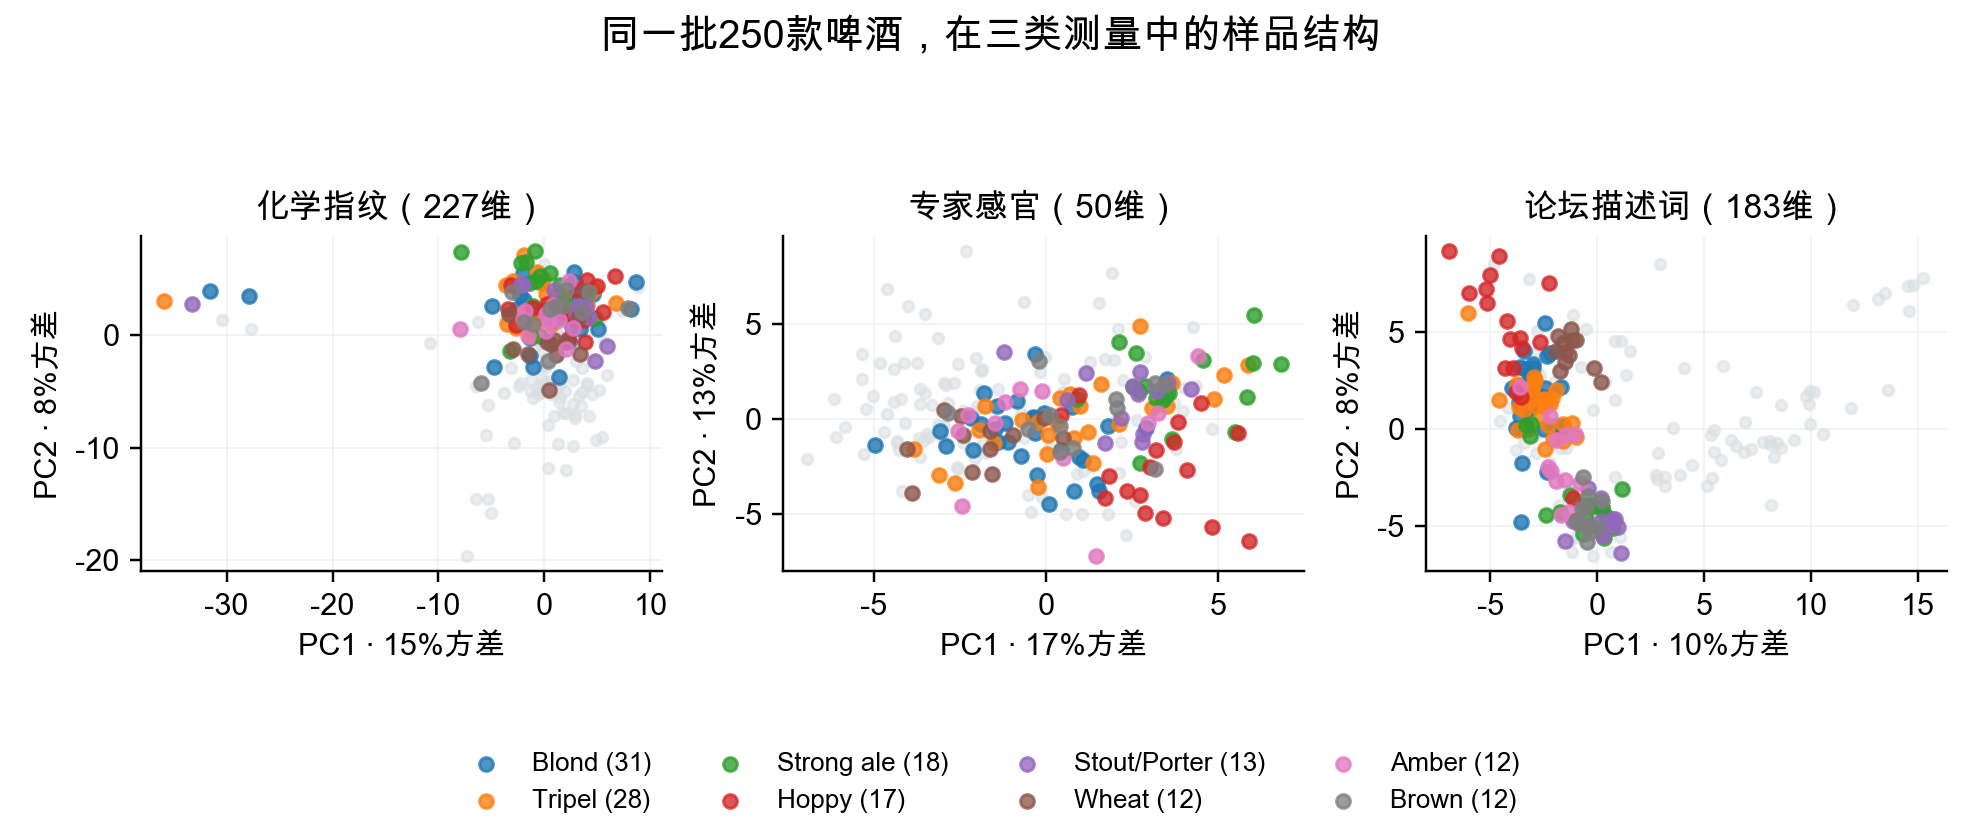
\includegraphics[width=.97\linewidth]{figures/beer_spaces.png}\caption{同一批250款啤酒在化学、专家感官与论坛词汇三个测量空间中的前两主成分。颜色标出样本最多的八种风格，其余样本为灰色；坐标仅表示各空间内部的主要变化方向，三幅图的轴不能直接互换。}\end{figure}

\section{统一建模路线}
\subsection{问题一：预测感官画像}
设化学向量为$\boldsymbol{x}_i$，连续感官画像为$\boldsymbol{y}_i\in\mathbb{R}^{50}$。采用八组极端随机树作为主模型，按感官语义分组共享树结构；逐指标梯度提升树与训练集均值作为对照。固定按风格分层的175/75训练—留出划分，超参数仅在训练集内五折选择。主指标为50个目标等权的宏平均RMSE：
\[
\mathrm{Macro\!-\!RMSE}=\frac1{50}\sum_{j=1}^{50}\sqrt{\frac1{75}\sum_{i=1}^{75}(y_{ij}-\hat y_{ij})^2}.
\]
模型选择依据连续感官预测；代理等级只用于展示，不宣称还原原始评分。
另预先指定15组语义直接对应的专家指标与论坛描述符，计算全样本Spearman相关，并对两侧分别按风格去均值后复算，以检查跨来源一致性是否仅由风格差异造成。论坛指标不参与专家模型训练、调参和化合物筛选。对附件7中183个非空评论描述符，使用同一175/75划分建立额外的化学到消费者语言模型。每列仅按训练集均值、标准差变换，采用固定参数的多输出极端随机树；以训练集内五折选择惩罚强度的Ridge作为对照。逐词统计相对训练均值基线的留出RMSE降幅，并计算去除风格均值后的留出排序相关。该任务预测的是评论用词的富集得分，不是消费者偏好。

\subsection{问题二：关联候选}
在211个化合物间计算Spearman相关，按$|\rho|\geq0.5$建共表达图，并保留边的正负方向。每个感官维度按
\[
S(c)=|\rho(c,y)|-0.35\max_{s\in A}|\rho(c,s)|
\]
逐步选取3个非完全冗余候选，其中$A$为已选集合。对样本进行500次重采样，报告候选入选频率及方向一致性。另计算风格校正后的关联，区分跨风格标志物与风格内仍存在的关联。网络结构不充当感官Top-3的前置筛选条件，化学知识只用于事后解释。

\subsection{问题三：条件生成与可行性}
对每个化合物分别生成检出状态和检出后的丰度。跨化合物依赖用总体秩变换后的收缩高斯Copula表示；各风格的检出率与丰度分位数向总体收缩。每种目标风格生成2000份候选谱，先筛去缺陷约束不满足及目标风格分类器不识别的谱，再在同一合格候选池内按目标典型性与源啤酒感官特点选出三份。以只追求目标典型性的筛选作为对照，并用另一种风格判别器与感官模型复核。真实目标参照可行性作为约束难度的辅助检查。

\section{实验与结果}
\subsection{预测性能}
\begin{table}[H]\centering\caption{75款留出样本上的感官预测}
\begin{tabular}{lrrrr}\toprule
模型&Macro-RMSE&Macro-MAE&$R^2$中位数&Spearman中位数\\\midrule
均值基线&0.5762&0.4205&-0.0066&--\\
八组极端随机树&0.4881&0.3475&0.1883&0.4158\\
逐指标梯度提升树&0.4880&0.3505&0.1833&0.3819\\\bottomrule
\end{tabular}
\end{table}
两种树模型的RMSE差仅0.0001，不据此断言算法优势。更有解释价值的是预测能力的差异：八组模型在Mouthfeel组相对均值基线降低33.3\%的RMSE，在Overall上仅降低4.5\%。因此应用时应先区分哪些感官目标有可用预测信号。
最终按已选参数在全部250款上重新拟合，交付250$\times$50连续画像及对应代理0--6等级表；表内值是全样本拟合后的应用输出，泛化误差只由前述75款留出样本估计。
\begin{figure}[H]\centering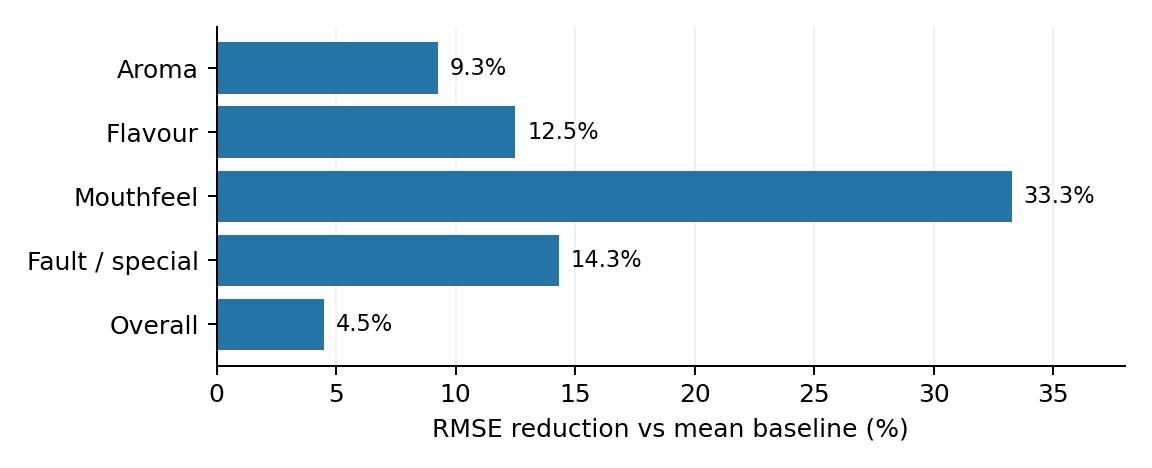
\includegraphics[width=.72\linewidth]{figures/q1_family_gain.png}\caption{化学指纹对不同感官组的留出预测改进。}\end{figure}
论坛描述符的额外预测中，极端随机树的183项目标RMSE降幅中位数为9.5\%，49项超过20\%；Ridge没有目标超过10\%。专家评分未单列的苹果味、苹果香和玉米香分别改善33\%、30\%、37\%，去除风格均值后的留出Spearman相关分别为0.35、0.31、0.36。因每风格留出样本较少，风格内结果仍是探索性证据。

\subsection{消费者评论的跨来源核验}
在15组预先指定的同义词对中，专家评分与论坛描述符在全部250款上的Spearman相关以酒精感（0.699）、苦味（0.645）、甜味（0.524）及麦芽滋味（0.506）较高；酯香（0.121）与双乙酰香（0.088）较低。按风格去均值后，酒精感与苦味分别降至0.330和0.381，麦芽滋味降至0.178，说明总体相关有明显的风格成分；甜味仍为0.487。该检验说明哪些专家感官维度能够在消费者语言中找到支持，不等于预测消费者喜好，也不把单词富集得分解释为感官强度。
\begin{figure}[H]\centering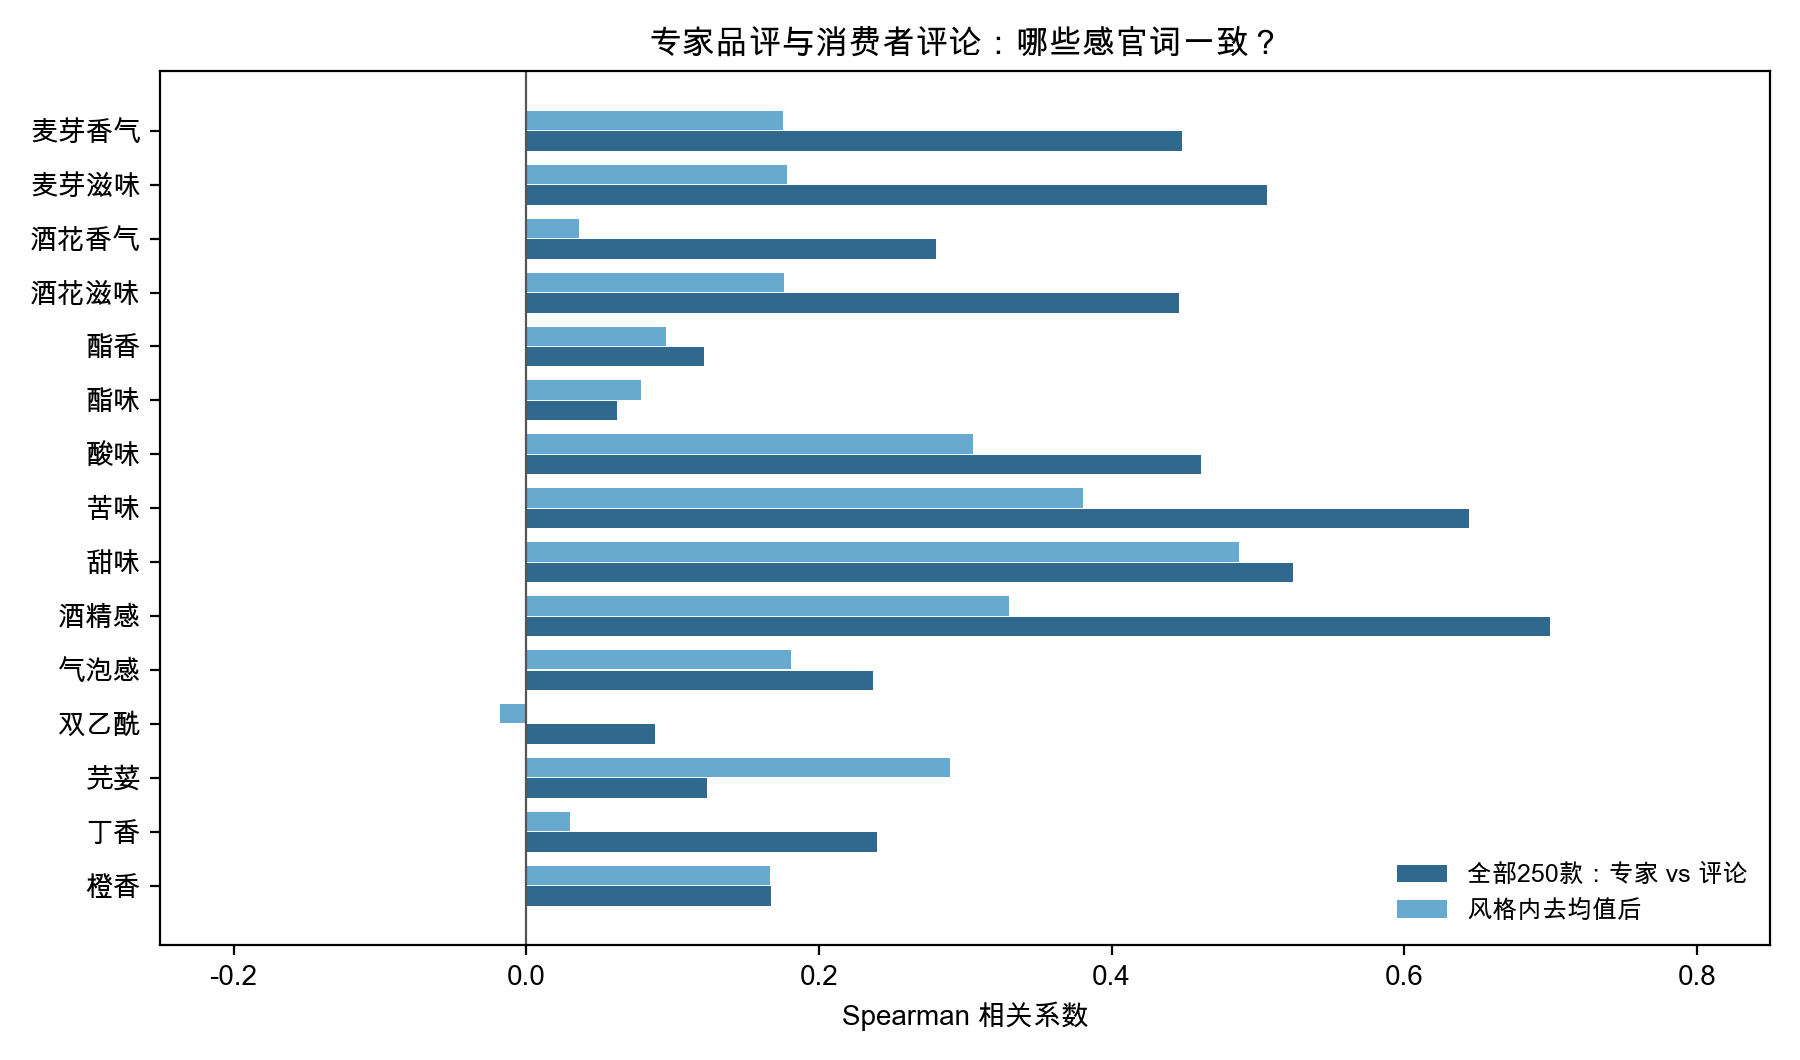
\includegraphics[width=.82\linewidth]{figures/expert_forum_bridge.png}\caption{15组专家评分与论坛评论描述符的对应。浅色条为分别按风格去均值后的相关。}\end{figure}

\subsection{关联网络与候选稳定性}
$|\rho|\geq0.5$时，共表达图有211个节点、564条边和44个孤立节点，最大连通分量含159个节点。规模最大的六个社区分别有39、37、22、20、20、17个化合物；例如17节点社区包含ethyl decanoate、ethyl hexanoate、ethyl octanoate等共同变化的酯类。图中将每个社区内化合物的标准化丰度取平均，再与15项代表性感官指标计算相关：第二社区在苦味和酒花味上较强，第六社区在酒体、气泡和苦味上较强。
\begin{figure}[H]\centering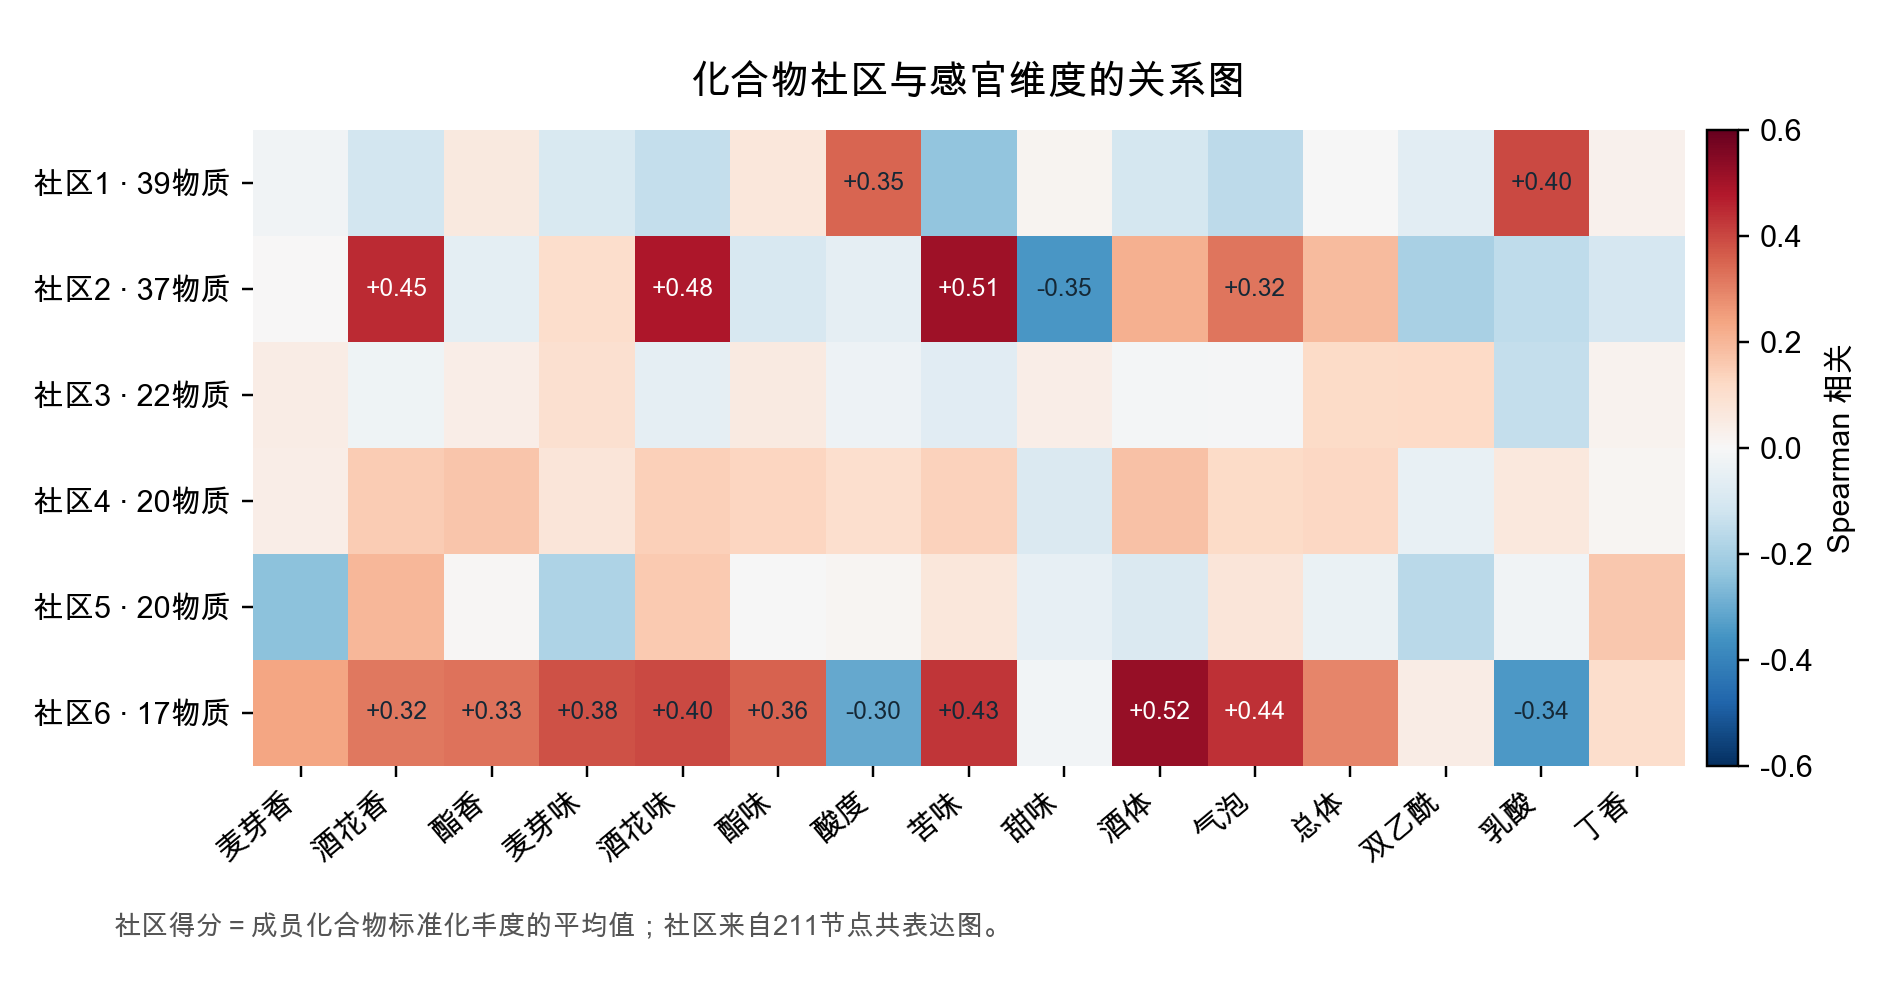
\includegraphics[width=.96\linewidth]{figures/module_sensory_map.png}\caption{化合物共表达社区与代表性感官维度的关系热力图。行是图上的化学社区，列是专家感官；颜色展示方向和强度，格中标出绝对值至少0.30的相关。}\end{figure}
这里的“社区”是化合物共变网络中连接较密的一组节点，先由化合物间相关定义，再看其与感官的对应；它既不是啤酒风格聚类，也不自动等于单一生化通路。表\ref{tab:communities}列出三个有清楚可读信息的社区；其余三个大社区在所示15项感官上的最大绝对相关均小于0.25。
\begin{table}[H]\centering\caption{主要化合物社区的组成与感官对应}\label{tab:communities}
\begin{tabular}{llp{5.2cm}l}\toprule
社区&主要来源&代表化合物&最明显的感官对应\\\midrule
1（39）&酵母16、麦芽9&1-octen-3-ol、ethyl phenylacetate&乳酸$+0.40$；酸度$+0.35$\\
2（37）&酒花21、酵母14&nerol oxide、alpha-calacorene&苦味$+0.51$；酒花味$+0.48$\\
6（17）&酵母15&ethyl decanoate、ethyl hexanoate、ethyl octanoate&酒体$+0.52$；气泡$+0.44$\\\bottomrule
\end{tabular}
\end{table}
在500次重采样中，50维共150个Top-3席位的入选频率中位数为0.324，其中28项达到0.6。首位候选通常比第二、第三位稳定。风格校正关联分析显示，50个维度中只有17个在最大单变量相关的首位保持不变，提示风格组成会改变解释顺序。
表中Top-3均称为待验证的关联候选；对风格内信号弱或重采样频率低的候选不作直接致香解释。
\begin{table}[H]\centering\caption{重算后有代表性的高频候选及解释层级}
\begin{tabular}{llrrl}\toprule
感官维度&候选化合物&相关方向及强度&入选频率&解释\\\midrule
X4vg&X4VG&$+0.473$&0.924&直接对应\\
F\_esters\_ethac&ethyl acetate&$+0.503$&0.976&酯类通路一致\\
A\_malt\_all&methylpyrazine&$+0.350$&0.670&麦芽反应类别一致\\
co2&ethyl octanoate&$+0.553$&0.990&工艺或风格代理\\\bottomrule
\end{tabular}
\end{table}
高入选频率表示候选在重采样中容易再次被选中；上表最后一行说明稳定的统计标志物仍可能缺少直接的感官机制。

\subsection{生成与迁移}
在固定175/75划分中，211个异风格源—目标组合有176组通过目标风格和缺陷门槛且留有至少30份候选。独立感官模型测得源引导组的特点距离为2.449，目标典型性对照为2.607；176组中有146组改善。按源啤酒聚类重采样，平均改善为0.168，95\%区间为$[0.132,0.206]$。代价是目标典型性下降。另一种风格判别器将68.6\%的源引导候选识别为请求风格；真实留出样本每风格仅3--8款，不能把分类器判断等同实际风格。
\begin{table}[H]\centering\caption{三种目标风格的真实留出参照与生成谱检查}
\begin{tabular}{lrrrrr}\toprule
目标风格&训练款数&留出款数&生成谱风格命中&留出谱风格命中&检出率误差\\\midrule
Tripel&20&8&71.7\%&50.0\%&0.092\\
Kriek&7&3&40.8\%&66.7\%&0.141\\
Lambic&8&3&54.7\%&100.0\%&0.128\\\bottomrule
\end{tabular}\end{table}
\begin{figure}[H]\centering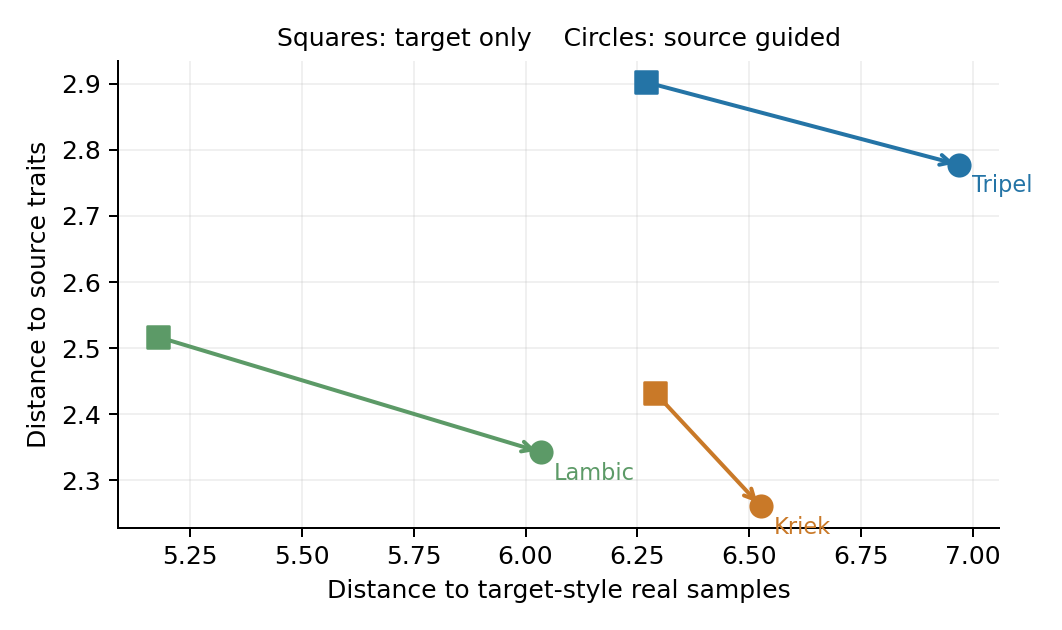
\includegraphics[width=.60\linewidth]{figures/q3_tradeoff.png}\caption{各目标风格中，源引导使源特点距离降低，同时增大到真实目标样本的距离；两轴均为越小越好。}\end{figure}
\begin{figure}[H]\centering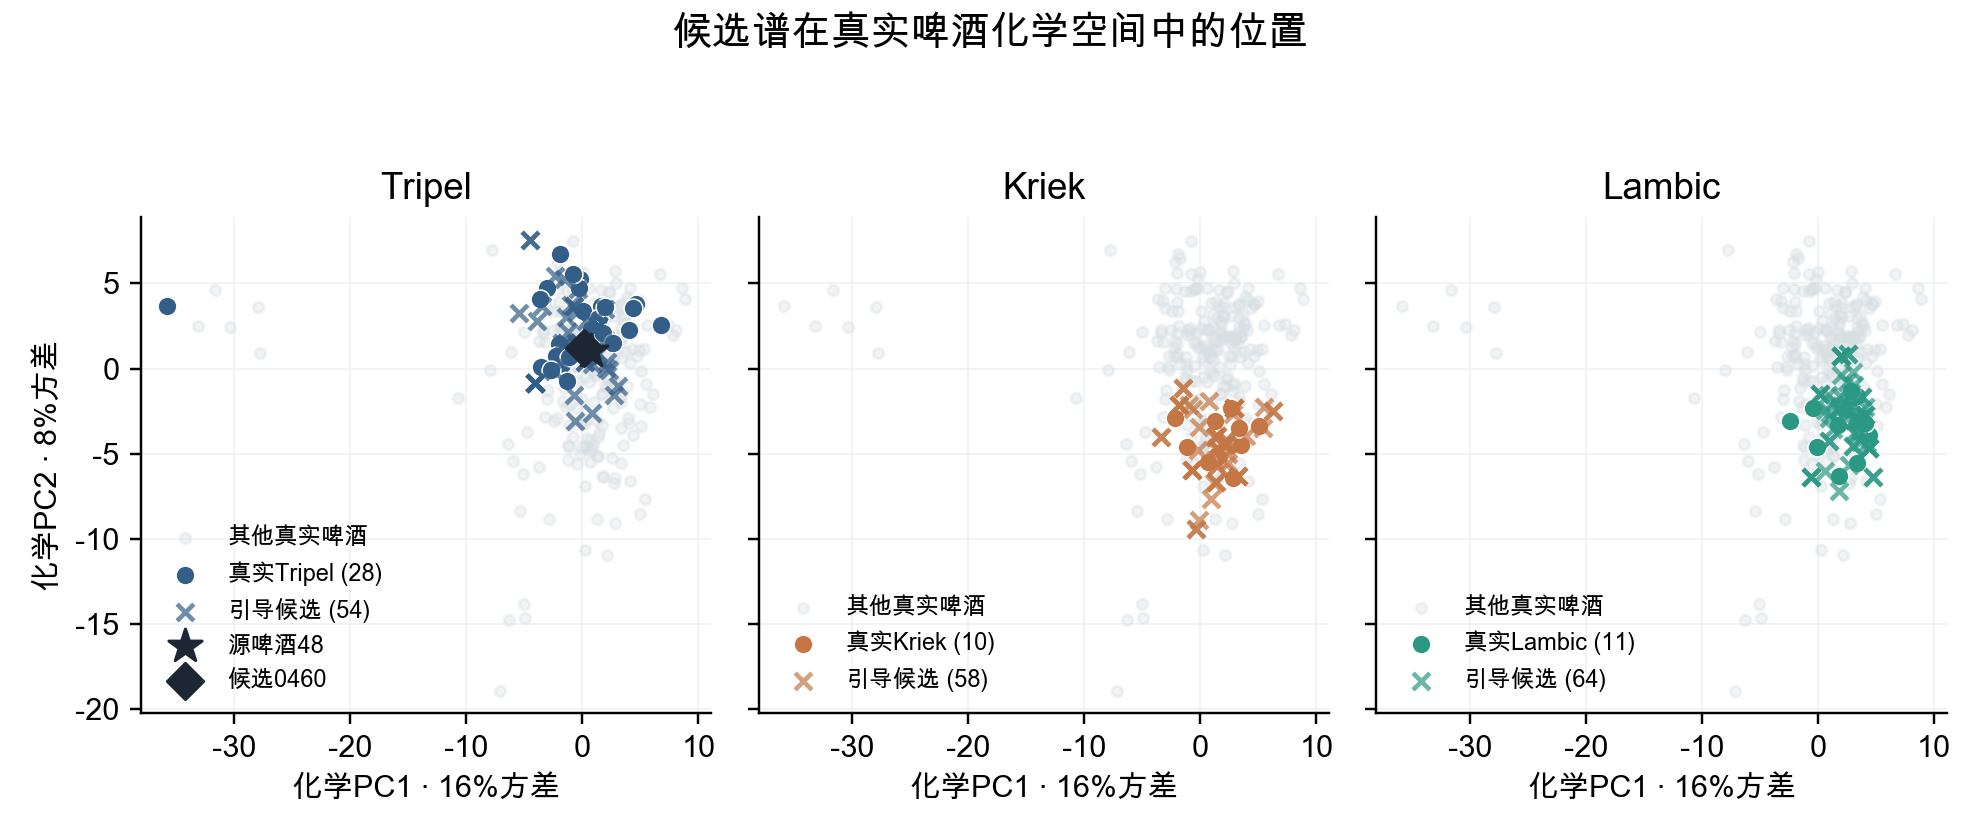
\includegraphics[width=.88\linewidth]{figures/candidate_chemical_space.png}\caption{三个目标风格的真实样本与选中候选在同一化学主成分空间的位置。灰点为其他真实啤酒，圆点为真实目标风格啤酒，叉号为引导候选；Tripel面板额外标出源样本48及其候选。}\end{figure}
严格要求四项缺陷化合物相对源啤酒均不增加时，11款留出Pils/Lager没有一款能在真实Tripel中找到满足条件的参照；按已知阈值放宽后仅1款可找到参照。

\noindent\textbf{结论：}化学指纹可预测部分专家感官与消费者描述词；共表达社区呈现不同的感官关联块，Top-3给出可验证的候选名单。两部分条件生成给出可检查的化学谱，源引导在多数可比较组合中保留更多源啤酒特点。稀有风格的可行性与实际可酿造性仍需品评验证。

\end{document}
